% TODO translate template
\documentclass{ufsctex/ufsctex}

\usepackage{amsmath, amsfonts, amsthm, makecell, mathtools, pdfpages, tikz}

% English captions
\addto\captionsbrazil{
	\renewcommand{\figurename}{Figure}
	\renewcommand{\tablename}{Table}
	\renewcommand{\listfigurename}{List of Figures}
	\renewcommand{\listtablename}{List of Tables}
	\renewcommand{\contentsname}{Table of Contents}
	\renewcommand{\bibname}{REFERENCES}
	\renewcommand{\proofname}{Proof.}
}
\makeatletter
\renewcommand{\listadeabreviaturas}{
	\pretextualchapter{List of Acronyms}\@starttoc{las}}
\renewcommand{\listadesimbolos}{
	\pretextualchapter{List of Symbols}\@starttoc{lsb}}
\renewcommand{\listadealgoritmos}{
	\pretextualchapter{List of Algorithms}\@starttoc{loa}}
\makeatother

% Use standard \mathcal font
\DeclareMathAlphabet{\mathcal}{OMS}{cmsy}{m}{n}

% Create theorem environments
\newtheorem{definition}{Definition}
\newtheorem{corollary}{Corollary}

% Tabular configurations
\renewcommand\theadfont{\bfseries}

% Cover info
\instituicao[a]{Universidade Federal de Santa Catarina}
\departamento[o]{Departamento de Informática e Estatística}
\curso[o]{Programa de Graduação em Ciência da Computação}
\documento[a]{Monografia}
\titulo{Reducing keys in Rainbow-like signature schemes}
\autor{Matheus Silva Pinheiro Bittencourt}
\grau{Bacharel em Ciência da Computação}
\local{Florianópolis}
\data{11}{Novembro}{2019}
\orientador[Orientador]{Prof.\ Ricardo Felipe Custódio, Dr.}
\coorientador[Coorientador]{Gustavo Zambonin, Bel.}
\coordenador[Coordenador]
	{Prof.\ José Francisco Danilo de Guadalupe Correa Fletes}
\numerodemembrosnabanca{2}
\orientadornabanca{nao}
\coorientadornabanca{nao}
\bancaMembroA{
	Prof. Daniel Panario, Dr.\\
	Carleton University
}
\bancaMembroB{
	Lucas Pandolfo Perin, Me.\\
	Universidade Federal de Santa Catarina
}

\dedicatoria{A Fátima, que infelizmente não pode acompanhar minha trajetória,
mas tenho certeza de que estaria orgulhosa.}

\agradecimento{Agradeço aos meus pais que me fizeram capaz de entender e
percorrer os caminhos do conhecimento e da vida. A toda a minha família que
nunca me faltou com apoio sempre que precisei, em especial ao meu padrinho
Fernando e a minha madrinha Daniela. Ao meu orientador Prof. Ricardo e ao Prof.
Daniel pela ajuda no desenvolvimento deste trabalho com as inúmeras e
produtivas reuniões. Ao Gustavo que me proporcionou a oportunidade de ser
orientado por um amigo, e que contribui enormemente para este trabalho. Ao
Douglas Silva e ao Douglas Martins que me orientaram em diversos aspectos da
vida acadêmica e profissional. A todos os amigos que fiz dentro e fora do
curso, que me acompanharam e me ajudaram direta ou indiretamente a percorrer
esse trajeto. Em especial, agradeço ao Lucas e ao Vinicius que sempre me
motivaram a vencer as batalhas enfrentadas com o ânimo e a dedicação
necessária. Por último, e com certeza não menos importante, agradeço ao Mateus
e ao Luís pela cumplicidade e companhia mesmo quando nada parecia bem, e por
todas as pessoas incríveis que eles me proporcionaram conhecer.}

\epigrafe{``\textit{Ce qui embellit le désert,
c'est qu'il cache un puits quelque part...}''}{Le Petit Prince}

\textoResumo{Os algoritmos clássicos de assinatura digital como RSA e ECDSA
baseiam sua segurança na dificuldade da fatoração de inteiros, e no logaritmo
discreto, respectivamente. Esses problemas já possuem algoritmos quânticos que
os resolvem em tempo polinomial, ou seja, com computadores quânticos poderosos
o suficiente, o uso dos algoritmos de assinatura digital mais difundidos
tornará-se impraticável. Naturalmente, com o aumento do poder computacional
quântico, o interesse por criptossistemas resistentes a ataques que utilizam-se
de tais computadores também cresceu. A área que estuda esses criptossistemas é
chamada de criptografia pós-quântica. Particularmente, esses algoritmos
baseiam-se numa série de problemas que permanecem difíceis, mesmo que
computadores quânticos poderosos sejam utilizados, logo, despertam o interesse
para substituir os criptossistemas clássicos. Este trabalho aborda
criptossistemas baseados em sistemas de polinômios multivariados, que,
baseiam-se em problemas como a solução de sistemas de polinômios e o
isomorfismo de polinômios, os quais ainda são resistentes a algoritmos
quânticos, e portanto, são candidatos para criptografia pós-quântica. Tais
esquemas possuem tamanhos de chaves muito maiores que os algoritmos clássicos.
Neste trabalho um novo método para redução de chaves privadas do esquema de
assinatura digital Rainbow é proposto. Usando este método as chaves privadas
podem ser reduzidas em até 84\%. Ainda, este método pode ser combinado com
outros de forma a reduzir o par de chaves por completo.}
\palavrasChave{criptografia pós-quântica, assinatura digital, Rainbow}

\textAbstract{Classic digital signature algorithms base their security upon the
difficulty of the integer factorization problem, and the discrete logarithm
problem, respectively. These problems already have quantum algorithms that
solve them in polynomial time, consequently, with sufficiently powerful quantum
computers, the use of the most common digital signature algorithms would become
impractical. Naturally, with the rise in quantum computational power, the
interest in cryptosystems resistant to attacks that make use of such computers
has raised as well. The area that studies such cryptosystems is called
post-quantum cryptography. Particularly, these algorithms are based upon a
series of problems that continue to be hard, even with quantum computers
available, hence, provoke interest to substitute the classical schemes. This
work approaches cryptosystems based on systems of multivariate polynomials.
They base their security upon problems like the polynomial system solving and
the isomorphism of polynomials, which are still resistant to quantum computers,
henceforth are candidates to post-quantum cryptography.  Such schemes have much
larger keys than classical algorithms. In this work a new method that allows
the reduction of private keys of the Rainbow digital signature scheme is
proposed. Using this method, private keys can be reduced by up to 84\%. Still,
this method can be combined with others to achieve smaller key pairs in their
entirety.}
\keywords{post-quantum cryptography, digital signatures, Rainbow}

\begin{document}

\pagenumbering{roman}
\capa{}
\pretextuais{}
\listadefiguras{}
\listadetabelas{}
\listadeabreviaturas{}
%\listadesimbolos{}
%\listadealgoritmos{}
\sumario{}

\chapter{Introduction}

Classic asymmetric cryptography is threatened as a result of the advance in
quantum algorithms development. The hardness of recovering private keys, for
instance, RSA\sigla{RSA}{Rivest-Shamir-Adleman} and ECDSA\sigla{ECDSA}{Elliptic
Curve Digital Signature Algorithm} keys, relies, respectively, on the hardness
of the integer factorization problem and the discrete logarithm problem.
Quantum polynomial-time algorithms that solve those problems already
exist~\cite{shor1999polynomial}. Using such algorithms, recovering private keys
can be done efficiently by a sufficiently powerful quantum computer. Hence, the
most used digital signature algorithms would become insecure.

In such a scenario, cryptosystems that run on classical computers and cannot be
broken by quantum computers should be used for handling digital signatures. The
area that studies such cryptosystems is called post-quantum cryptography, and
the interest in this has emerged with the development of quantum computers. The
security of these algorithms relies on problems that are not known to be
solvable in polynomial-time, therefore, they appear to be good candidates for
use in a scenario of attackers equipped with quantum computers.

There are several classes of post-quantum cryptosystems proposed in the
literature, and each of them relies on one kind of hard problem. This work aims
to study Multivariate Public-Key Cryptosystems
(MPKCs)\sigla{MPKCs}{Multivariate Public-Key Cryptosystems} based on Rainbow.
These cryptosystems are constructed using multivariate polynomials systems. A
polynomial system is usually composed of polynomial equations with single
variable monomials, and can be easily solved using, for instance, Gaussian
elimination. However, with the inclusion of more variables into the monomials,
it becomes a multivariate system. The problem of solving multivariate systems
is NP-Hard~\cite{garey1979npc}. Therefore, it may be interesting to build
cryptosystems based on this trait.

Several digital signature schemes were developed based on the structure of
multivariate systems. One of the first schemes presented was the Oil and
Vinegar\sigla{OV}{Oil and Vinegar} signature scheme~\cite{patarin1997ov}, which
was broken by Kipnis and Shamir in its original
specification~\cite{kipnis1998cryptanalysis}. A subsequent
work~\cite{kipnis1999unbalanced} reparametrized it, leading to a scheme called
Unbalanced Oil and Vinegar.\sigla{UOV}{Unbalanced Oil and Vinegar} The trapdoor
introduced in the original OV is used in many other schemes. In essence, they
are similar to OV but ended up optimizing the signature, and key sizes, while
maintaining security levels. These schemes are still considered secure.

MPKCs have very efficient signature generation and verification algorithms, as
well as small signatures, in some cases, smaller than classic algorithms. The
main caveat of such schemes is that they have large public and private keys.
Various efforts were made to reduce such parts of these cryptosystems, but, to
the best of our knowledge, none of them reduced both public and private keys.
This work aims to understand the Rainbow signature scheme, its subsequent
optimized schemes and the key reduction techniques proposed in the literature.
Finally, a new framework that allows for a reduction of both the private and
the public keys in Rainbow-like schemes is proposed.

\section{Goals and scope}

\textit{General goal:} Study and describe Rainbow-like digital signature
schemes, understand the optimizations that reduce keys and signature sizes, and
their impact on the security of the classic schemes. Observe and analyze the
impact of parameter selection for such algorithms, as this plays an important
role in efficient and fast implementations of the schemes. Analyze the
state-of-the-art schemes, to understand the strategies being used to optimize
the cryptosystems.

\textit{Specific goals:} Describe the classic OV and the UOV digital signature
schemes; Describe the Rainbow signature scheme; Introduce relevant
optimizations on Rainbow, like CyclicRainbow~\cite{petzoldt2010cyclicrainbow};
Compare and analyze the performance of the aforementioned schemes in terms of
operations needed to generate and verify signatures as well as storage
requirements. Finally, propose new optimizations on top of those schemes.

\textit{Scope:} This work will be focused on the Rainbow digital signature
scheme, its ancestors, and the optimizations made on top of it. Other classes
of post-quantum algorithms such as code-, lattice- and hash-based cryptosystems
will not be covered. Classical asymmetric algorithms will not be covered as
well. Quantum algorithms will also not be discussed.

\section{Methodology}

The work will be developed using the infrastructure and resources provided by
the Computer Security Laboratory (LabSEC/UFSC). A literature review will be
made to determine the state-of-the-art in MPKCs. Recently proposed schemes will
be studied, as well as broken ones for a better understanding of the
constructions used that optimize the classic multivariate schemes. The
performance of all the schemes studied should be observed along with the impact
of the optimizations.

\chapter{Cryptographic primitives}

In this chapter some basic cryptographic primitives will be described for a
complete understanding of the following chapters. All definitions and
descriptions are based on \cite{stinson2005cryptography}.

\section{Public Key Cryptography}

Symmetric cryptography consists of ciphering and deciphering a message with the
same key. This can be very useful if two parties, say Alice and Bob, have
agreed upon using the same key using a secure channel. But if Alice and Bob are
distant and do not have a secure channel to share a symmetric key, this cannot
be used. Public key cryptography resolves this issue, as there exists two keys.
One of the keys is public, everyone can have access, and it is used to encrypt
a message. The other key is private and can be held only by its owner, no one
else can access it. Deciphering a message can only be made with the private
key. Also, getting the private key from the public key should be
computationally unfeasible. Now, if Bob wants to send a private message to
Alice, he gets her public key through any channel of communication, encrypts
the message, and sends it to Alice. Alice, which possesses the private key, is
the only one capable of decrypting Bob's message.

The idea of public key cryptosystems was first introduced
in~\cite{diffie1976new}, but the first practical scheme of such kind was only
proposed in~\cite{rivest1977digital}. These algorithms can be thought as a
trapdoor one-way function, i.e. the encryption process ``traps'' the message,
and only with the possession of the private key, one can untangle the original
message from the trap. The security of these algorithms rely on the difficulty
of getting the private key from the public one, that is, it should be hard to
unravel the message from the trap.

\section{Digital Signatures}

Conventional signatures are used everyday to provide authenticity of documents,
like letters and contracts. A digital signature is a signature to a digital
document, that can be transmitted across a digital medium. Digitally signed
documents have considerable differences to conventional signatures. First, a
digital signature is not physically bonded to the signed document.  Second, the
verification procedure of the signature is distinct. Conventional signatures
are verified by similarity to other signatures that are trusted. Digital
signatures are verified using publicly known algorithms. Also, a digital
signature can be copied several times, and it will remain authentic. Care
should be taken, such that a document is not used more times than it should be.
For instance, a signed document saying that Alice wants to transfer some amount
of money to Bob should be used only once, as Bob could force the bank to
transfer this same amount multiple times. Adding the time the signature was
made to the signed document can mitigate this problem.

A digital signature scheme is composed of three efficient\footnote{Can be
computed in a reasonable time by the parties involved.} algorithms:

\begin{itemize}

	\item \textbf{Key generation:} Alice generates a key pair, publishes the
	public key to anyone who wants to verify her signatures, and keeps the
	private key secret.

	\item \textbf{Signature generation:} Alice, possessing the private key,
	signs a document $d$, yielding a signature $\sigma$, and publishes the pair
	$(d, \sigma)$. For each different document, a different signature will be
	produced.

	\item \textbf{Signature verification:} Bob wants to verify Alice's
	signature $(d, \sigma)$. With the public key, Bob can verify that, indeed,
	only Alice's private key could generate $\sigma$ for $d$. If someone
	altered $d$ to insert malicious information and sent this modified document
	$d'$, to Bob, the signature $\sigma$ would not be verified by the
	verification algorithm.

\end{itemize}

This can be seen as the inverse of sending private messages using public key
cryptography, as the owner of the private key ciphers the message to be signed.
Recall that it should be hard to find the private key from the public one, thus
it is hard to forge new signatures without possessing the private key.

A secure digital signature scheme should provide three properties to the signed
documents, as long as they are valid:

\begin{itemize}

	\item \textbf{Integrity:} The document is untouched compared to the
	originally signed document. Flipping one bit of the document would render
	the signature invalid.

	\item \textbf{Authenticity:} Only the owner of the private key can generate
	valid signatures for the corresponding public key. So, if a document is
	signed, it could only be signed be the private key owner. Generating new
	signatures, without the private key, should be computationally unfeasible
	for secure schemes.

	\item \textbf{Non-repudiation:} The signer cannot deny having created a
	valid signature $\sigma$ for a document $d$. This is due to the fact that,
	it is unfeasible to forge signatures.

\end{itemize}

\section{Cryptographic Hash Functions}

In the scope of this work, a hash function is a function that is used to map
arbitrarily sized data to a fixed length value, \text{i.e.} $\mathcal{H}:\{0,
1\}^* \rightarrow \{0, 1\}^n$. Such functions are useful to maintain integrity
of documents, for instance, a document $d$ has this fingerprint $h =
\mathcal{H}(d)$, which can be verified whenever one wants to ensure that $d$
was not modified. If for some reason the document was changed, this modified
version $d'$ would have a different fingerprint $h' = \mathcal{H}(d')$, and the
integrity of the original document would not be verified because $h \ne h'$.

Of course, due to the ``compression'' made by $\mathcal{H}$, there ought to
exist two documents that generate the same fingerprint, that is $h =
\mathcal{H}(d_1) = \mathcal{H}(d_2)$ and $d_1 \ne d_2$. This happens due to the
fact that there exists infinitely more documents than fingerprints, so by the
pigeonhole principle there will be infinitely many documents with the same
fingerprint. This can be a problem, because the integrity of those documents
could be erroneously verified. However, in practice, for secure hash functions,
this will happen with negligible probability for a large enough $n$.

Hash functions are extensively used in digital signatures. It enables the
algorithms to sign arbitrarily big documents by signing only the fingerprint
$h$. However, a hash function should satisfy some properties to be considered
cryptographically secure. Specially, three problems should be unfeasible to
solve. Let $\mathcal{H}:X \rightarrow Y$ be a hash function:

\begin{itemize}

	\item \textbf{Preimage:} Given $y \in Y$, find $x \in X$ such that $y =
		\mathcal{H}(x)$.

	\item \textbf{Second preimage:} Given $x \in X$, find $x' \in X,\; x' \ne
		x$ such that $\mathcal{H}(x) = \mathcal{H}(x')$.

	\item \textbf{Collision:} Find $x,\; x' \in X$ such that $\mathcal{H}(x) =
		\mathcal{H}(x')$.

\end{itemize}

Suppose that Alice is using $\mathcal{H}$ to sign a document $d$, this is,
Alice only signs $h = \mathcal{H}(d)$. If a malicious party, namely Eve, could
solve any of the preimage problems efficiently, let's say, Eve finds $d'$ such
that $h = \mathcal{H}(d) = \mathcal{H}(d')$ so she could publish the same
signature yielded by Alice as a valid signature for $d'$ without Alice's
private key. If Eve solves the collision problem efficiently, she could hand
Alice a document $d$ to be signed, while having generated a document with
malicious content $d'$. The signature created by Alice would be valid for both
$d$ and $d'$.

\section{Finite Fields}

These section's definitions are based on \cite{lidl1983encyclopedia}, and a
basic understanding of the algebraic structures used in multivariate schemes is
given.

\begin{definition}
A group $(G, *)$ with the set $G$ and the binary operation $*$ satisfies the
following conditions:
\begin{itemize}
	\item $*$ is associative, that is, $a*(b*c) = (a*b)*c$ for any $a, b, c \in
	G$.
	\item There exists an identity element $e \in G$ such that $a * e = e * a =
	a$.
	\item There exists an inverse for every $a \in G$ such that $a*a^{-1} =
	a^{-1}*a = e$.
\end{itemize}
If the group also satisfies the condition $a*b = b*a$ for all $a, b \in G$ then
it is called an abelian or commutative group.
\end{definition}

\begin{corollary}
The set of integers modulo $n$, denoted $\mathbb{Z}/n$, along with the ordinary
addition, form a finite abelian group denoted $\mathbb{Z}_n$.
\end{corollary}

\begin{proof}
The associativity and commutativity come from the regular addition operation.
The identity element is $0$ and the inverse element of any $a \in \mathbb{Z}/n$
is $-a \mod n$. $(\mathbb{Z}/n, +)$ is an abelian group.
\end{proof}

\begin{definition}
A ring $(R, +, *)$ with the set $R$ and the two binary operations $+$ and $*$
satisfies the conditions:
\begin{itemize}
	\item $(R, +)$ forms an abelian group.
	\item $*$ is associative, that is, $a*(b*c) = (a*b)*c$ for any $a, b, c \in
	R$.
	\item $*$ is distributive, that is, $a*(b+c) = a*b + a*c$ for any $a, b, c
	\in R$.
\end{itemize}
\end{definition}

It must be emphasized that not only the ordinary multiplication and addition
can be used to form groups or rings.

\begin{definition}
A ring $(R, +, *)$ can be further classified as:
\begin{itemize}
	\item \textbf{Commutative} if $*$ is commutative, that is, $a*b = b*a$ for
	all $a, b \in R$.
	\item A \textbf{division ring} if the nonzero elements of $R$ form a group
	under $*$.
	\item A \textbf{field} if it is a commutative division ring.
\end{itemize}
\end{definition}

\begin{corollary}
The set of integers modulo a prime $p$, denoted $\mathbb{Z}/p$, along with the
ordinary addition and multiplication, form a finite field denoted
$\mathbb{F}_p$.
\end{corollary}

\begin{proof}
As stated above $(\mathbb{Z}/n, +)$ is an abelian group, therefore
$(\mathbb{Z}/p, +)$ is a commutative group as well. The ordinary multiplication
is associative, distributive and commutative. Now it must be shown that
$(\mathbb{Z} - \{0\}, *)$ forms a group. The identity element of this group is
$1$. $a*b$ will never be zero because if $a*b \equiv 0 \mod p$ then either $a$
or $b$ is zero and divides $p$, which is a contradiction because $p$ is prime.
Now to show that all elements have inverses, the Bézout's identity can be used.
For every $a \in \mathbb{Z}/p$ there exists $x, y \in \mathbb{Z}/p$ such that
$a*x + p*y \equiv 1 \mod p$, due to the fact that $\text{gcd}(a, p) = 1$. Note
that $p*y \equiv 0 \mod p$, hence $a*x \equiv 1 \mod p$ and $x$ is the inverse
of $a$. $(\mathbb{Z}/p, +, *)$ is a finite field.
\end{proof}

\begin{definition}
Given a ring $(R, +, *)$ there exists a positive integer $n$ such that $n*r =
0$ for every $r \in R$. The least such positive integer is called the
characteristic of $n$. If $n$ does not exist, the characteristic of $R$ is $0$.
\end{definition}

It can be noted that finite fields have prime characteristic. If a finite field
had a characteristic $n = p*q$ with $p, q \in \mathbb{Z}$ and $1 < p,q < n$,
then $n*e = (p*q)*e = 0$ would be true and the ring would not be a division
ring, because multiplying two nonzero elements cannot result in $0$.

\begin{corollary}\label{cor:extension}
Let $\mathbb{F}_p[x]/f(x)$ be the set of polynomials with coefficients in a
finite field $\mathbb{F}_p$, modulo an irreducible polynomial\footnote{An
irreducible polynomial cannot be divided by a polynomial other than $f(x) =
1$.} $f(x)$ of degree $n$. $\mathbb{F}_p[x]/f(x)$ along with the ordinary
polynomial addition and multiplication modulo $f(x)$, form an extension field
denoted $\mathbb{F}_{p^n}$.
\end{corollary}

For illustration, the finite field $\mathbb{F}_{2^2}$ can be defined with its
elements being $P = \{0, 1, x, x+1\}$, and the operations, the ordinary
addition and multiplication of polynomials modulo $f(x) = x^2 + x + 1$. Note
that all coefficients are in $\mathbb{F}_2$. The addition operation is given by
the Table \ref{tab:addition} and the multiplication by Table
\ref{tab:multiplication}. The addition in $\mathbb{F}_{2^2}$ is the trivial
polynomial addition with coefficients modulo $2$, and there is no need for
polynomial reductions. The multiplication though needs reductions modulo the
irreducible polynomial. For instance, $x*(x+1) \equiv x^2+x \equiv 1 + 1*f(x)
\equiv 1 \mod f(x)$.

\begin{table}
\begin{center}
\begin{tabular}{c|cccc}
$+$   & $0$   & $1$   & $x$   & $x+1$ \\
\hline
$0$   & $0$   & $1$   & $x$   & $x+1$ \\
$1$   & $1$   & $0$   & $x+1$ & $x$   \\
$x$   & $x$   & $x+1$ & $0$   & $1$   \\
$x+1$ & $x+1$ & $x$   & $1$   & $0$   \\
\end{tabular}
\caption{Addition operation of $\mathbb{F}_{2^2}$}
\label{tab:addition}
\end{center}
\end{table}

\begin{table}
\begin{center}
\begin{tabular}{c|cccc}
$*$   & $0$ & $1$   & $x$   & $x+1$ \\
\hline
$0$   & $0$ & $0$   & $0$   & $0$   \\
$1$   & $0$ & $1$   & $x$   & $x+1$ \\
$x$   & $0$ & $x$   & $x+1$ & $1$   \\
$x+1$ & $0$ & $x+1$ & $1$   & $x$   \\
\end{tabular}
\caption{Multiplication operation of $\mathbb{F}_{2^2}$}
\label{tab:multiplication}
\end{center}
\end{table}

\begin{proof}
To prove Corollary \ref{cor:extension} the field properties should hold for the
finite fields of this fashion. Let $P = \mathbb{F}_p[x]/f(x)$. $(P, +)$ forms
an abelian group with $e = 0$ and the inverse of any $a \in P$ being $-a$.
Also, $(P - \{0\}, *)$ forms a group, with the identity element being $1$. The
inverse element of any $a \in P - \{0\}$ can be found using Bézout's indentity
because $\text{gcd}(a, f(x)) = 1$, this comes from the fact that $f(x)$ is
irreducible. So, there exists $x, y \in P - \{0\}$ such that $a*x + f*y \equiv
1 \mod f(x)$, hence $x$ is the inverse of $a$. Observe that $a*b \equiv 0 \mod
f(x)$ never happens in the group $(P - \{0\}, *)$, because either $a$ or $b$
would need to be zero and would divide $f(x)$, which is a contradiction because
$f(x)$ is irreducible. All other properties can be trivially extended from the
ordinary polynomial addition and multiplication. $(P, +, *)$ is a finite field.
\end{proof}

Extensions of the binary field $\mathbb{F}_2$ are specially interesting because
representing and operating with them can be very computationally efficient. An
element of $\mathbb{F}_{p^n}$ needs $n$ elements of $\mathbb{F}_p$ to be
represented, hence an element of $\mathbb{F}_{2^8}$ needs $8$ bits, or $1$
byte. For instance, the element $x^7 + x^5 + x + 1 \in \mathbb{F}_{2^8}$ can be
represented by the binary $8$-uple $(1, 0, 1, 0, 0, 0, 1, 1)$. The addition,
when elements are represented in such way, is simply the bitwise exclusive or
XOR operation. The multiplication operation can be performed efficiently using
a modification to the Peasant's algorithm, which takes advantage of the binary
representation. The reduction modulo $f(x)$ can also be done by a series of
bitwise XOR operations. For small finite fields, a lookup table such as Table
\ref{tab:addition} and \ref{tab:multiplication}, can be precomputed in order to
dramatically improve the efficiency of the operations, as only one query to
such table would be needed to obtain the result.

\chapter{Multivariate cryptography}

In this chapter, basic foundations are given for the comprehension of the
techniques proposed in the current work. Section \ref{sec:mqsystems} contains a
description of the basic mathematical structure used to build MPKCs. Section
\ref{sec:bipolar} presents the construction used in the schemes discussed in
this work. Section \ref{sec:problems} depicts the underlying problems in which
MPKCs rely their security on. Section \ref{sec:mqschemes} describes the schemes
addressed in this study. Section \ref{sec:rainbowvariants} illustrates some
variants of the Rainbow digital signature scheme present in the literature.
Section \ref{sec:equivalentkeys} demonstrates a method to find equivalent
private keys in Rainbow-like schemes and how it can be used to reduce the outer
maps.

\section{Systems of multivariate equations}\label{sec:mqsystems}

Standard polynomials are simply a sum of monomials, each monomial consists of a
variable and a constant that multiplies it. Polynomials can be represented
using a vector that stores those constants. With multivariate polynomials, each
monomial consists of a multiplication of more than one variable and, again, a
constant. This inclusion of multiple variables to the monomials is what makes
them interesting to use in cryptosystems, since solving a system of such
polynomials is computationally hard. For the purpose of multivariate
cryptography, multivariate quadratic equations are sufficient, hence most
commonly used.

\begin{definition}
A multivariate quadratic polynomial is defined as:
\begin{equation}
p(x_1,\dots,x_n) = \sum_{i=1}^n \sum_{j=i}^n \alpha_{ij} x_i x_j +
	\sum_{i=1}^n \beta_i x_i + \gamma
\end{equation}
where all $x, \alpha, \beta, \gamma \in \mathbb{F}$
\end{definition}

A system of polynomials is a set of polynomials that share the same variables.
It is known that, for polynomials with $n$ variables, systems that have at
least $n$ polynomials may be solvable, and the existence of solutions can be
checked efficiently. One of the most common methods for solving such systems is
the Gaussian elimination. Note that, not all systems with $n$ polynomials and
$n$ variables have a unique solution, some of them may even have infinitely
many solutions. It happens due to the fact that a polynomial can be linearly
dependent of others in the systems.

Systems of multivariate polynomials can be constructed as well. Opposed to the
systems explained above, solving multivariate systems is a NP-Hard
problem~\cite{garey1979npc}, even for the simplest case of quadratic
polynomials, therefore they are interesting to be used in building
cryptosystems. Specially, systems of multivariate quadratic polynomials will be
used, as the addition of more variables to the monomials does not increase the
hardness of the problem.

These systems can be seen as maps. For instance, a system $\mathcal{P}$, with
$n$ variables and $m$ equations, defines a map $\mathcal{P}:\mathbb{F}^n \to
\mathbb{F}^m$. Applying this map over a vector of variables consists of
substituting these variables into the equations and taking their results as the
output of the map.

\begin{definition}\label{def:mqsystem}
A system $\mathcal{P}$ of multivariate quadratic polynomials is defined as:
\begin{equation}\label{eq:mqsystem}
\begin{split}
p^{(1)}(x_1,\dots,x_n) &= \sum_{i=1}^n \sum_{j=i}^n \alpha^{(1)}_{ij} x_i x_j
	+ \sum_{i=1}^n \beta^{(1)}_i x_i + \gamma^{(1)} \\
p^{(2)}(x_1,\dots,x_n) &= \sum_{i=1}^n \sum_{j=i}^n \alpha^{(2)}_{ij} x_i x_j
	+ \sum_{i=1}^n \beta^{(2)}_i x_i + \gamma^{(2)} \\
&\vdotswithin{=} \\
p^{(m)}(x_1,\dots,x_n) &= \sum_{i=1}^n \sum_{j=i}^n \alpha^{(m)}_{ij} x_i x_j
	+ \sum_{i=1}^n \beta^{(m)}_i x_i + \gamma^{(m)}
\end{split}
\end{equation}
where all $x, \alpha, \beta, \gamma \in \mathbb{F}$
\end{definition}

Each equation of the system can be represented as an upper triangular square
matrix of order $n+1$, where the element on the $i$-th line and the $j$-th
column represents the constant that multiplies the monomial $x_i x_j$. The last
column is used to represent the linear terms and the constant term. The $k$-th
polynomial of the system is represented by a matrix of the form:

\begin{equation}\label{eq:matrixrepresentation}
A^{(k)} =
\begin{pmatrix}
\alpha^{(k)}_{11} & \alpha^{(k)}_{12} & \alpha^{(k)}_{13} & \cdots &
	\alpha^{(k)}_{1n} & \beta^{(k)}_1 \\
0 & \alpha^{(k)}_{22} & \alpha^{(k)}_{23} & \cdots &
	\alpha^{(k)}_{2n} & \beta^{(k)}_2 \\
0 & 0 & \alpha^{(k)}_{33} & \cdots &
	\alpha^{(k)}_{3n} & \beta^{(k)}_3 \\
\vdots & \vdots & \vdots & \ddots & \vdots & \vdots \\
0 & 0 & 0 & \cdots & \alpha^{(k)}_{nn} & \beta^{(k)}_n \\
0 & 0 & 0 & \cdots & 0 & \gamma^{(k)} \\
\end{pmatrix}
\end{equation}

Furthermore, $p^{(k)}$ may be written as:
\begin{equation}
p^{(k)}(x_1,\cdots,x_n) =
	(x_1,\cdots,x_n,1) \cdot A^{(k)} \cdot (x_1,\cdots,x_n,1)^T
\end{equation}

Systems of multivariate quadratic equations can be represented and stored with
ease, as shown above. It is worth recalling that the coefficients of those
equations are elements in a small finite field, thus operating with them is
computationally efficient. Although easy to manipulate, storing these matrices
is not space efficient. A notable effort resulted in various works that reduce
the public map, e.g. \cite{petzoldt2010cyclicrainbow}, or the private map, e.g.
\cite{yasuda2012reducing}, but none of them reduced the key pair
simultaneously.

With the keys represented as matrices, some works introduce special structures
into these matrices, in such a way that representing them requires less space.
For instance, the series of works by Petzoldt et al., introduce a framework
that enables the public key to be partially selected. Such selection is done in
a way that some special structure is introduced into the matrices, hence
reducing their space requirements. Notably, CyclicRainbow uses a cyclic
structure in the matrix representation of the public key.

\section{Bipolar construction}\label{sec:bipolar}

The basic construction used in multivariate cryptosystems is based on the
composition of multiple transformations. As described above, a multivariate
system, as per Definition \ref{def:mqsystem}, may be used as a function
$\mathcal{F}:\mathbb{F}^n\to\mathbb{F}^m$. The central transformation of this
construction will be a system of such kind, which will contain some specific
structure such that, one can find preimages. $\mathcal{F}$ will remain secret,
and with the combination of one or more affine transformations, a public system
of equations, with no apparent structure, will be generated.

As shown in Figure \ref{fig:bipolar}, the bipolar construction consists of
three secret maps, and a public map that is derived from these three.
$\mathcal{P}$ and $\mathcal{F}$ are multivariate systems. $\mathcal{S}$ and
$\mathcal{T}$ are random invertible affine maps. In the signing procedure,
$\mathcal{F}^{-1}$ means finding one of possibly many preimages, and
$\mathcal{F}$ introduces some structure that allows one to do such. The affine
maps take care of hiding this structure by actually scrambling the variables of
the system. When generating the keys, one calculates $\mathcal{P}$ by the
composition of the secret maps $\mathcal{P} = \mathcal{S} \circ \mathcal{F}
\circ \mathcal{T}$.

\begin{figure}
\centering
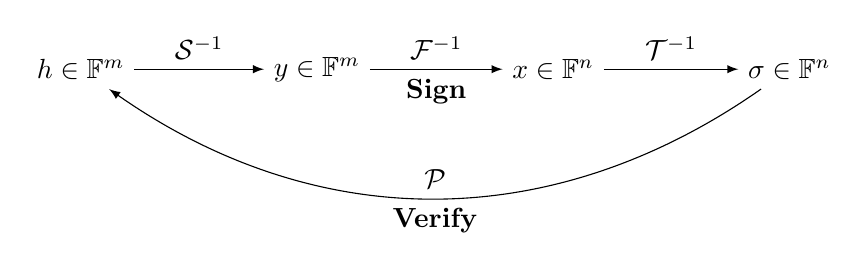
\begin{tikzpicture}
\node (h) at (0, 0) {$h \in \mathbb{F}^m$};
\node (y) at (3, 0) {$y \in \mathbb{F}^m$};
\node (x) at (6, 0) {$x \in \mathbb{F}^n$};
\node (z) at (9, 0) {$\sigma \in \mathbb{F}^n$};
\draw[-latex] (h) -- node[above]{$\mathcal{S}^{-1}$} (y);
\draw[-latex] (y) --
node[above]{$\mathcal{F}^{-1}$} node[below]{\textbf{Sign}} (x);
\draw[-latex] (x) -- node[above]{$\mathcal{T}^{-1}$} (z);
\draw[-latex] (z) to[bend left=35] node[above]{$\mathcal{P}$}
node[below]{\textbf{Verify}} (h);
\end{tikzpicture}
\caption{Flow of the bipolar construction}\label{fig:bipolar}
\end{figure}

Note that $n \geq m$ should hold when using the construction for digital
signature schemes. This makes the public map $\mathcal{P}$ surjective, and
ensures that for every hash $h \in \mathbb{F}^m$ there exists a signature
$\sigma \in \mathbb{F}^n$. Encryption schemes can be constructed too, in this
case $n \leq m$ should hold, thus making the map injective and ensuring that
the decryption process outputs only one plain text.

With a hash function $\mathcal{H}:\{0,1\}^* \to \mathbb{F}^m$ one can sign a
document $d$ by calculating $h = \mathcal{H}(d)$. As shown in Figure
\ref{fig:bipolar}, recursively compute the signature $\sigma =
\mathcal{T}^{-1}(\mathcal{F}^{-1}(\mathcal{S}^{-1}(h)))$. This is possible due
to the fact that those maps are constructed such that they can be inverted. To
verify the signature $\sigma$ for document $d$ one can simply check if $h =
\mathcal{P}(\sigma)$ holds.

\section{Underlying computational problems}\label{sec:problems}

This section describes the problems in which multivariate cryptosystems
security rely on.

\subsection{Polynomial system solving}\label{sec:posso}

Solving systems of polynomials is the basic underlying problem, since, solving
the public system is sufficient to forge new signatures.

\begin{definition}
Polynomial System Solving problem: given a system $\mathcal{P}$ as per Equation
\ref{eq:mqsystem}, find a vector $x' = (x_1',\cdots,x_n')$ such that
$p^{(1)}(x') = p^{(2)}(x') = \cdots = p^{(m)}(x') = 0$.
\end{definition}

This problem was proven to be NP-Hard~\cite[Appendix A7.2]{garey1979npc} even
for the simplest case of quadratic polynomials over $\mathbb{F}_2$. The special
case of this problem where the polynomials have degree 2 is called
\textbf{MQ-Problem}. The NP-Hardness of this problem is important due to the
fact that, it is not feasible for an attacker to solve the public map
$\mathcal{P}$ directly, hence not feasible to forge signatures this way.

\subsection{Isomorphism of polynomials}

The security of multivariate cryptosystems, due to their construction, usually
does not rely exclusively on the MQ-Problem. An attacker knows that the public
map is constructed by the composition of the private maps, thus one can try to
decompose the map $\mathcal{P}$ into three maps, isomorphic to the private
ones, and forge new signatures. The problem of finding such isomorphic maps is
called the Extended Isomorphism of Polynomials problem.

\begin{definition}
Extended Isomorphism of Polynomials problem: given a nonlinear multivariate
system $\mathcal{P} = \mathcal{S} \circ \mathcal{F} \circ \mathcal{T}$ with
$\mathcal{F}$ belonging to some class $\mathcal{C}$ of special nonlinear
systems that can be inverted. Find $\tilde{\mathcal{S}}$, $\tilde{\mathcal{F}}$
and $\tilde{\mathcal{T}}$ such that $\mathcal{P} = \tilde{\mathcal{S}} \circ
\tilde{\mathcal{F}} \circ \tilde{\mathcal{T}}$ and $\tilde{\mathcal{F}} \in
\mathcal{C}$.
\end{definition}

With $\tilde{\mathcal{S}}$, $\tilde{\mathcal{F}}$ and $\tilde{\mathcal{T}}$ one
may forge a signature for a document $d$ by computing $\sigma =
\tilde{\mathcal{T}}^{-1}(\tilde{\mathcal{F}}^{-1}(\tilde{\mathcal{S}}^{-1}(
\mathcal{H}(d))))$ and publish it as a valid signature for the public key
$\mathcal{P}$. Recall that $\tilde{\mathcal{F}} \in \mathcal{C}$ so it can be
inverted.

Some variations of the problem with only one affine map or even ones that
involve finding the original central map $\mathcal{F}$ exist, but the extended
variation is the most generic one. In fact, solving the problem as stated
above, in polynomial time, is enough to break the Rainbow Signature
Scheme~\cite{ding2005rainbow} submitted to the NIST Post-Quantum Cryptography
Standardization Process~\cite{ding2017nist}.

Opposed to the MQ-Problem, the hardness of this problem is not well
established. Actually, on the balanced Oil and Vinegar
scheme~\cite{patarin1997ov} decomposing the public map was done efficiently by
~\cite{kipnis1998cryptanalysis}. While this problem remains an open problem,
security proofs for multivariate schemes based on the bipolar construction will
be absent. Still, MQDSS\sigla{MQDSS}{Multivariate Quadratic Digital Signature
Scheme}~\cite{chen20165} is a provably secure multivariate cryptosystem,
however it is based on a totally different construction.

\section{Multivariate digital signature schemes}\label{sec:mqschemes}

This section contains a description of the main schemes that are based on the
bipolar construction.

\subsection{Oil and Vinegar}\label{sec:ov}

The original Oil and Vinegar signature scheme was presented by
\cite{patarin1997ov}. It introduces a trapdoor that is based upon the idea of
having two sets of variables in the central map, called oil and vinegar. The
central map is constructed in such a way that the polynomials are linear in the
oil variables, that is, there are no monomials with two oil variables. With
this fact in mind, when generating a signature, one may actually linearize the
central system and solve for oil variables. A detailed description of the Oil
and Vinegar signature scheme follows.

Let $K$ be a small finite field, e.g. $\mathbb{F}_2$. Let $o$ and $v$ be
integers, such that $o$ is the number of oil variables and $v$ the number of
vinegar variables. Let $O$ be the set of oil variables and $V$ the set of
vinegar ones. Let $\mathcal{H}: \{0,1\}^* \to K^o$ be a cryptographic hash
function.

The private key consists of two maps $\mathcal{T}$ and $\mathcal{F}$. Let
$\mathcal{T}: K^{o+v} \to K^{o+v}$ be a random \textit{invertible} affine
transformation, its effect is to rewrite every variable as a linear combination
of all other variables. This map will be used to hide the structure of the
central map. Let $\mathcal{F}: K^{o+v} \to K^{o}$ be the central map, composed
of $o$ equations of the form:

\begin{equation}\label{eq:ovpolynomial}
y^{(k)} =
\underbrace{\sum_{i=1}^{v}\sum_{j=i}^{v} \alpha^{(k)}_{ij} x_i x_j}_{
V \times V} +
\underbrace{\sum_{i=v+1}^{v+o}\sum_{j=1}^{v} \beta^{(k)}_{ij} x_i x_j}_{
O \times V} +
\underbrace{\sum_{i=1}^{o+v} \gamma^{(k)}_{i} x_i}_{\text{linear}} +
\underbrace{\delta^{(k)}}_{\text{constant}}
\end{equation}

where $x_1,\dots,x_v \in V$ are the ``vinegar'' variables and
$x_{v+1},\dots,x_{v+o} \in O$ are the ``oil'' variables. Note that the oil
variables are not multiplied between themselves, this will be important to find
preimages for this map when signing a message.

The public map $\mathcal{P}$ is a simple composition of the secret maps,
$\mathcal{P} = \mathcal{F} \circ \mathcal{T}$. Both $\mathcal{F}$ and
$\mathcal{P}$ are multivariate systems. $\mathcal{F}$ has the special structure
mentioned above, nevertheless $\mathcal{P}$ looks randomly built. With these
maps described, let the public/private key pair be
$(\mathcal{P},(\mathcal{F},\mathcal{T}))$.

To sign a document $d$, compute its hash value $h = \mathcal{H}(d)$ and find a
preimage $(x_1,\dots,x_{o+v})$ for the map $\mathcal{F}$ such that
$(y^{(1)},\dots,y^{(o)}) = (h_1,\dots,h_o)$. Recall the structure present in
$\mathcal{F}$, setting random values to the vinegar variables makes the system
linear. Hence, finding a preimage consists of selecting vinegar variables at
random, substitute them into $\mathcal{F}$, and find the oil variables through
Gaussian elimination. If the system cannot be solved, new vinegar variables
need to be chosen. The vector of variables $x$ are found such that
$\mathcal{F}(x)=h$. Next, using the map $\mathcal{T}$ the signature itself may
be computed. Recall that $\mathcal{T}$ is invertible, thus $\mathcal{T}^{-1}$
can be obtained. With both maps inverted, the signature $\sigma$ of $d$ is
published as $\sigma = \mathcal{T}^{-1}(x)$.

To verify a signature $\sigma$ of a document $d$, one can simply check if
$\mathcal{P}(\sigma) = \mathcal{H}(d)$ holds, therefore the signature is valid,
otherwise it is invalid. The equality does actually hold for valid signatures,
as $\mathcal{P}$ is a composition of the maps that were inverted in the signing
procedure. Recall that $\mathcal{P}$ is a system of multivariate equations,
hence hard to solve.

\subsection{Unbalanced Oil and Vinegar}

The original Oil and Vinegar explained in Section \ref{sec:ov} is actually
insecure due to the fact that $o = v$. It is called Balanced Oil and Vinegar
due the same amount of oil and vinegar variables. This aspect of the
cryptosystem was exploited by~\cite{kipnis1998cryptanalysis}, where a method
was introduced to efficiently forge new signatures when $o = v$. The same
authors subsequently proposed a new scheme, called Unbalanced Oil and
Vinegar~\cite{kipnis1999unbalanced}. This work proposes new parameters for the
original OV. The most common instantiation of this new scheme is the $v = 2o$
case.

\subsection{Rainbow}\label{sec:rainbow}

The Rainbow signature scheme was proposed in~\cite{ding2005rainbow}. It can be
described simply as a multilayered UOV. Actually, it is a generalization of the
UOV scheme, in other words, UOV is a single layer Rainbow instantiation. This
newly proposed scheme greatly improves space requirements in comparison to UOV.
Both public and private key sizes, as well as signatures size, are reduced for
equivalent security levels. A detailed description of the Rainbow cryptosystem
follows.

Each layer of this so called Rainbow will has its own polynomials, as well as
its own set of oil and vinegar variables. These polynomials have the same
structure as OV polynomials, but the layers are intrinsically connected when
constructed. Namely, $V_l$ and $O_l$ are respectively the set of vinegar
variables and the set of oil variables of the $l$-th layer. Let $u$ be the
number of layers. Let $v_1, v_2, \cdots, v_{u+1}$ be the number of vinegar
variables in each layer, such that $0 < v_1 < v_2 < \cdots < v_{u+1} = n$. Note
that the layers actually grow bigger, this is due to the fact that each set of
vinegar variables contains the vinegar variables from the previous layer, that
is $V_1 \subset V_2 \subset \cdots \subset V_{u}$. As you go deeper into the
layers, the oil variables become vinegar variables, \textit{i.e.} $V_{l+1} =
V_l \cup O_l$. Keep in mind that $|V_l| = v_l$ and $|O_l| = o_l = v_{l+1} -
v_{l}$.

The connection between variables of the layers exist in such a way that the
layers have to be inverted one after the other for the complete inversion of
the central map. To start this process, one randomly selects the first set of
vinegar variables and substitutes them, making the first layer linear. Recall
that the oil variables of some layer are part of the vinegar variables of the
subsequent layer. When the first layer is solved, the set $O_1$ can be used to
construct $V_2$ in its entirety. With known values for $V_2$ one can linearize
the second layer and solve it. Repeating this process for every layer, inverts
the whole central map. It may happen that some layer will not be solvable, in
this case, a new set $V_1$ is chosen and the inversion process starts over.
This happens with very small probability as shown in Section
\ref{sec:invertibility}.

Let the sets $V_l = \{x_1, \cdots, x_{v_l}\}$ be the vinegar variables of the
$l$-th layer, and $O_l = V_{l+1} - V_l$ the respective oil variables. Recall
that, each layer $l$ has $o_l = v_{l+1} - v_{l}$ equations, and thus $o_l$
equations are needed to solve for $O_l$ variables. For each layer $l$,
construct a system $\mathcal{F}_l$ composed of $o_l$ polynomials of the form:

\begin{equation}\label{eq:rainbowmap}
y^{(k)} =
\sum_{i=1}^{v_l}\sum_{j=i}^{v_l} \alpha^{(k)}_{ij} x_i x_j +
\sum_{i=v_l+1}^{v_{l+1}}\sum_{j=1}^{v_l} \beta^{(k)}_{ij} x_i x_j +
\sum_{i=1}^{v_{l+1}} \gamma^{(k)}_{i} x_i +
\delta^{(k)}
\end{equation}

for $k = v_l, \cdots, v_{l+1} - 1$ and $l = 1, \cdots, u$. Observe that the
polynomials are Oil and Vinegar polynomials, just like the ones in
Equation~\ref{eq:ovpolynomial}, and they can be solved for $O_l$ when $V_l$ has
known values. Let the central map $\mathcal{F}:K^{n} \to K^{n-v_1}$ be the
union of the $u$ layers. To hide the central map, two random invertible affine
maps will be used. Let $\mathcal{S}:K^{n-v_1} \to K^{n-v_1}$ and
$\mathcal{T}:K^{n} \to K^{n}$ be part of the private key. Publish $\mathcal{P}
= \mathcal{S} \circ \mathcal{F} \circ \mathcal{T}$ as the public key.

Let $\mathcal{H}: \{0,1\}^* \to K^{n-v_1}$ be a cryptographic hash function. To
sign a document $d$, compute $h = \mathcal{H}(d)$. Compute $y = (y_1, \cdots,
y_{n-v_1}) = \mathcal{S}^{-1}(h)$. Solve all layers of $\mathcal{F}$ using the
process described above, in order to find $x = (x_1, \cdots, x_n)$ such that
$\mathcal{F}(x) = y$. Finally, publish $\sigma = \mathcal{T}^{-1}(x)$ as the
signature for $d$.

Verifying a signature $\sigma$ for a document $d$ is as simple as checking if
$\mathcal{P}(\sigma) = \mathcal{H}(d)$ holds. Recall that, again, $\mathcal{P}$
is a multivariate system that appears to be randomly built, thus hard to solve
directly.

For illustration, Table \ref{tab:rainbowkeysizes} shows a comparison between
the key sizes of some Rainbow instances proposed in \cite[Chapter
6]{petzoldt2013thesis}. Let $m = n - v_1$ be the number of equations in Rainbow
central and public maps. The private and public key sizes of Rainbow-like
signature schemes are given, respectively, by the formulas:

\begin{equation}\label{eq:rainbowprivatekeysize}
K_{pr} =
\underbrace{m^2 + m}_{\mathcal{S}} + \underbrace{n^2 + n}_{\mathcal{T}} +
\underbrace{\sum_{l=1}^{u} o_l \left(
\frac{v_l(v_l + 1)}{2} + v_l o_l + v_{l+1} + 1
\right)}_{\mathcal{F}}
\end{equation}

\begin{equation}
\begin{split}
K_{pu} &= m \left( \frac{n (n + 1)}{2} + n + 1 \right) \\
&= m \frac{(n+1)(n+2)}{2}
\end{split}
\end{equation}

These can be easily checked by looking at Equation \ref{eq:rainbowmap} and the
size of the affine maps $\mathcal{S}$ and $\mathcal{T}$. Also, the public key
size is simply the size of a multivariate system with $n$ variables and $m$
equations. The public key size formula can be checked by observing Equation
\ref{eq:matrixrepresentation}, as the public map is composed of $m$ matrices of
such kind. With $u=1$, OV and UOV key sizes can be calculated using $K_{pr}$
and $K_{pu}$ also, as Rainbow is a generalization of the Oil and Vinegar
schemes.

\begin{table}
\begin{center}
\begin{tabular}{|c|c|c|c|}
\hline
% header
\thead{Security level\\(bits)} & \thead{Parameters\\$(K, o_1, v_1, v_2)$}
& \thead{Private key size\\(bytes)} & \thead{Public key size\\(bytes)} \\
\hline
% data
80  & $(\mathbb{F}_{256}, 17, 17, 9)$   & 19208   & 25740   \\ \hline
100 & $(\mathbb{F}_{256}, 26, 22, 11)$  & 45450   & 60390   \\ \hline
128 & $(\mathbb{F}_{256}, 36, 28, 15)$  & 103704  & 139320  \\ \hline
192 & $(\mathbb{F}_{256}, 63, 46, 22)$  & 440638  & 596904  \\ \hline
256 & $(\mathbb{F}_{256}, 85, 63, 30)$  & 1086971 & 1498230 \\ \hline
\end{tabular}
\caption{Rainbow key sizes for parameters proposed in \cite{petzoldt2013thesis}}
\label{tab:rainbowkeysizes}
\end{center}
\end{table}

\section{Rainbow variants}\label{sec:rainbowvariants}

The cryptosystems described above have a notable space requirement. For
instance, the Rainbow public key can get up to 1.6 MB for secure
parameters~\cite[Table 2]{ding2017nist} in comparison to ECDSA's 64 bytes
public keys. This section presents some variants in the literature that reduce
Rainbow key sizes. It is shown that, all of them reduce either the public map
or the private central map, but not both.

\subsection{Establishing a linear relation between public and private maps}
\label{sec:relation}

In~\cite{petzoldt2010cyclicrainbow} an approach is used in such a way that one
can partially select the public key. It relies on an important aspect of the
schemes previously discussed. In the UOV case, it is demonstrated that the
secret map $\mathcal{S}$ actually establishes a linear relation between the
private and public coefficients of the equations. This makes it possible to
select $\mathcal{P}$ and $\mathcal{S}$ in a clever manner, such that their
representations are smaller, introducing some kind of structure like a
circulant matrix in the case of CyclicRainbow.

Recall the UOV construction of the maps $\mathcal{P} = \mathcal{F} \circ
\mathcal{T}$. To better understand this linear relation, the equations can be
simplified, without its linear and constant terms. Let $n = o + v$, and the
$k$-th private polynomial of the system, without its linear and constant terms,
be denoted as:

\begin{equation}
y^{(k)} = \sum_{r=1}^n \sum_{s=r}^n\left(\alpha^{(k)}_{rs}x_rx_s\right)
\end{equation}

Let $\mathcal{T} \in K^{n \times n}$ be the matrix that describes the secret
affine map. The $k$-th public polynomial can be written as:

\begin{equation}\label{eq:pubpolynomial}
p^{(k)} = \sum_{r=1}^n \sum_{s=r}^n
\left[ \alpha^{k}_{rs} \sum_{i=1}^n(t_{ir}x_i) \sum_{j=1}^n(t_{js}x_j) \right]
\end{equation}

where $t_{ij}$ is the element of $\mathcal{T}$ in the $i$-th line and the
$j$-th column. The inner summations come from the matrix multiplication
operation, where the vector of $x$ variables is multiplied with $\mathcal{T}$
when the map is applied, giving a ``new'' vector of $x$ variables, that are
actually just linear combinations of the old ones. Let the public polynomial be
denoted similarly to the private one:

\begin{equation}
p^{(k)} = \sum_{r=1}^n \sum_{s=r}^n \left( \rho^{(k)}_{rs}x_rx_s \right)
\end{equation}

To establish a relation between $\alpha_{rs}$ and $\rho_{rs}$
observe the structure of Equation \ref{eq:pubpolynomial} where $\alpha_{rs}$ is
multiplying two polynomials. Expanding the inner summations gives:

\begin{equation}
(t_{1r}x_1 + t_{2r}x_2 + \cdots + t_{nr}x_n)
(t_{1s}x_1 + t_{2s}x_2 + \cdots + t_{nr}x_n)
\end{equation}

This can be described as a new polynomial with quadratic terms, applying
distributive multiplication:

\begin{equation}\label{eq:tau}
\sum_{i=1}^{n}\sum_{j=i}^n \left( \tau^{rs}_{ij} x_i x_j \right)
\quad \mathrm{where:} \quad \tau^{rs}_{ij} =
\begin{cases}
	t_{ir} t_{is} &\mbox{if } i=j \\
	t_{ir} t_{js} + t_{jr} t_{is} &\mbox{otherwise}
\end{cases}
\end{equation}

Substituting Equation \ref{eq:tau} into Equation \ref{eq:pubpolynomial} yields:

\begin{equation}
p^{(k)} = \sum_{r=1}^n \sum_{s=r}^n
\left[
\alpha^{k}_{rs} \sum_{i=1}^{n}\sum_{j=i}^n \left( \tau^{rs}_{ij} x_i x_j \right)
\right]
\end{equation}

Therefore, a relation between private and public coefficients can be written as:

\begin{equation}\label{eq:relation}
\rho^{(k)}_{ij} = \sum_{r=1}^{n}\sum_{s=r}^n
\left( \tau^{rs}_{ij} \alpha^{k}_{rs} \right)
\end{equation}

After randomly choosing $\mathcal{S}$, Equation \ref{eq:relation} depicts the
linear relation between the public ($\rho$) and private ($\alpha$)
coefficients. Hence one can choose and fix $\rho$ and find $\alpha$ using this
equation. Observe that not all public coefficients can be chosen, otherwise no
structure would be present in $\mathcal{F}$ and it could not be inverted. This
could also be used to recalculate $\mathcal{F}$ from $\mathcal{P}$ and
$\mathcal{S}$. The idea behind this relation is further expanded to Rainbow key
pairs, and is described in detail by~\cite{petzoldt2011small}. This relation
was extensively used to reduce either public or private keys, but not both.
Reducing key sizes with this strategy consists of introducing some structure
into one part of the key, such that its representation becomes smaller, and
calculating the other part using the equations above. Notable key optimizations
will be briefly discussed hereafter.

\subsection{CyclicRainbow}

CyclicRainbow~\cite{petzoldt2010cyclicrainbow} uses the relations explained in
Section~\ref{sec:relation} to structure the public key. In the key generation
step, parts of the public key matrix representation are selected such that they
form a circulant matrix.

\begin{definition}
A square circulant matrix of order $n$ is of the form:
\begin{equation}
A =
\begin{pmatrix}
a_1     & a_2    & \cdots  & a_{n-1} & a_n     \\
a_n     & a_1    & a_2     & \cdots  & a_{n-1} \\
a_{n-1} & a_n    & a_1     &         & a_{n-2} \\
\vdots  &        & \ddots  & \ddots  & \vdots  \\
a_2     & \cdots & a_{n-1} & a_n     & a_1
\end{pmatrix}
\end{equation}
\end{definition}

Such matrices allow for a compact representation. Storing the vector $(a_1,
a_2, \cdots, a_n)$ is enough to represent the matrix completely, as its
elements form a structured repetition. Introducing this structure in parts of
the public key, when possible, reduces the representation of the public system
significantly. In fact this method allows a public key reduction factor of up
to 2.9, for secure parameters. This repetition of elements also leads up to a
repetition of operations when verifying a signature. Exploiting this common
field multiplications leads to a reduction factor of up to 2.4 in the number of
operations needed to evaluate the public map, \textit{i.e.} to verify a
signature \cite[Table 10.3]{petzoldt2013thesis}.

\subsection{RainbowLRS2}

RainbowLRS2~\cite[Section 9.2]{petzoldt2013thesis} introduces matrices
generated by Linear Recurring Sequences into the public key, just like in
CyclicRainbow. To generate an $m \times n$ matrix of this type, a vector $a =
(a_1, a_2, \cdots, a_m) \in \mathbb{F}^m$ of distinct elements is selected.
The $i$-th row of this matrix is:

\begin{equation}\label{eq:lrsmatrix}
A[i] = (a_i^0, a_i^1, a_i^2, \dots, a_i^{n-1}) \qquad i = 1, \dots, m
\end{equation}

Storing the vector $a$ is sufficient the represent the matrix $A$, since every
row can be calculated using Equation \ref{eq:lrsmatrix}. Using matrices of this
fashion in the public map representation, allows for a reduction factor of up
to 3.1. Veritably, this method is similar to the one used in CyclicRainbow,
thus provides an akin improvement in space requirements. The main difference is
that CyclicRainbow uses rotations to generate each row. In RainbowLRS2 the rows
are defined by equation \ref{eq:lrsmatrix}. It is shown
in~\cite{petzoldt2013thesis} that field multiplications also repeat in the
verification process of RainbowLRS2, which allows for a speed up to a factor of
2.2~\cite[Table 10.3]{petzoldt2013thesis}.

\subsection{Circulant Rainbow}

Circulant Rainbow~\cite{peng2017circulant} introduces circulant matrices in the
central private map, in contrast to CyclicRainbow that does it on the public
map. These circulant relations will be present in very specific parts of the
central polynomials, precisely in the terms that have oil variables. Throughout
the signature generation, after inserting values into the vinegar variables,
one will have to solve a linear system as shown in Section \ref{sec:rainbow}.
Due the structure introduced in the coefficients of the central map, this
system will be represented by a circulant matrix. Solving such systems can be
done more efficiently using a method described in~\cite{peng2017circulant}.
Indeed, the private key needs less space to be represented. Circulant Rainbow
has a private key 1.8 times smaller than the original Rainbow, and the
signature generation can be 2.9 times faster if the optimized method for
solving the special linear systems is used instead of the Gaussian elimination.
Notably, \cite{hashimoto2018security} discourages the use of Circulant Rainbow.
It is shown that the Kipnis-Shamir's attack~\cite{kipnis1998cryptanalysis} can
be used to recover equivalent Circulant Rainbow private keys in polynomial
time.

\subsection{NC-Rainbow}

NC-Rainbow~\cite{yasuda2012reducing} proposes the use of non-commutative rings
instead of a finite field in the central map. Further, isomorphisms between the
rings and the fields are used in the composition of the public map. Through
this isomorphism it can be shown that a NC-Rainbow central map is equivalent to
the original Rainbow central map. In fact, it is stated that an element
$\alpha$ of a non-commutative ring $R$ can be represented by $r$ elements in
the finite field $K$. This smaller representation of the elements in $R$ is
what leads to a more compact representation of the central map. Indeed, it is
shown that the use of this technique can reduce the private key by a factor of
4 and sign documents with 1.6 times less field multiplications with the
proposed parameters for the new scheme.

In~\cite{thomae2012quo}, it is shown that NC-Rainbow is just a special case of
introducing structures into the private central map. Additionally, it is
demonstrated that, the reduction of NC-Rainbow to the original Rainbow is not
enough to prove security. The reduction in the opposite direction is needed and
is absent in the original work. The existent reduction just provides an upper
bound for the security of the new scheme. Actually, known attacks on Rainbow
were sensibly improved for the NC-Rainbow case. The optimizations reduce the
MinRank attack complexity from $2^{288}$ to $2^{192}$ and for the HighRank, the
reduction is from $2^{128}$ to $2^{96}$. Hence, the usage of non-commutative
rings in the central map is not recommended, as it greatly decreases the
security of the original Rainbow.

\section{Equivalent keys in Multivariate Cryptosystems}
\label{sec:equivalentkeys}

In~\cite{wolf2005equivalent} is introduced the idea of equivalent keys for
Multivariate Cryptosystems. Equivalent keys are different private keys that
lead to the same public key. They can be found using the idea of
``sustainers''. Sustainers are transformations that do not alter the property
present in the central map that allow its inversion. For instance, a sustainer
to UOV is a transformation that, when applied to the central map, does not
change the fact that oil variables do not multiply themselves. By letting
$\Delta, \Gamma$ be sustainers, an equivalent key can be found using the
equation:

\begin{equation}\label{eq:sustainer}
\mathcal{P} =
\underbrace{\mathcal{S} \circ \Delta^{-1}}_{\mathcal{S'}}
\circ
\underbrace{\Delta \circ \mathcal{F} \circ \Gamma}_{\mathcal{F'}}
\circ
\underbrace{\Gamma^{-1} \circ \mathcal{T}}_{\mathcal{T'}}
\end{equation}

The maps $\mathcal{S'}, \mathcal{F'}, \mathcal{T'}$ are equivalent keys for
$\mathcal{P}$. If for every $\mathcal{S}$ and $\mathcal{T}$, $\Delta$ and
$\Gamma$ can be found such that $\mathcal{S'}$ and $\mathcal{T'}$ contain some
special structure, the private key space can be reduced.

For instance, if this idea is applied to UOV, additive sustainers can be used
to reduce the storage requirements of $\mathcal{T}$. An additive sustainer only
adds a term to the constant term. This sustainer clearly does not break the Oil
and Vinegar property of the central map, and it can be used to subtract the
constant terms in $\mathcal{T}$. Let $\mathcal{T}$ be a random affine map,
$\Gamma^{-1}$ can be chosen such that it subtracts all its constant terms. So,
for every $\mathcal{T}$, there exists an equivalent map $\mathcal{T'}$ that has
no constants. Using this fact, $\mathcal{T}$ can be chosen without its
constants already.

Other sustainers are presented in~\cite{wolf2011equivalent}. For instance,
Gauss sustainers can be used to further reduce the private key space. These
sustainers are transformations that permute or add rows and columns of a matrix
and they can be described by invertible matrices. Again, let $\Gamma$ be a
sustainer for UOV:

\begin{equation}
\Gamma(x) =
\begin{pmatrix}
A & 0 \\
B & C \\
\end{pmatrix} \cdot x
\end{equation}

such that $A \in K^{v \times v}_q$, $B \in K^{o \times v}_q$, $C \in K^{o
\times o}_q$ and $A, C$ are invertible. Recall that $x$ is the column vector of
variables in the central equations. $\Gamma$ only shuffles the vinegar
variables within themselves, so it is in fact a sustainer. The construction of
Equation \ref{eq:sustainer} can be applied as:

\begin{equation}
\begin{split}
\mathcal{P} &= \mathcal{F} \circ \Gamma \circ \Gamma^{-1} \circ \mathcal{T} \\
&=
\mathcal{F} \circ
% Gamma inverse
\begin{pmatrix}
A & 0 \\
B & C \\
\end{pmatrix}
\circ
% Gamma
\begin{pmatrix}
A^{-1} & 0 \\
-C^{-1} \cdot B \cdot A^{-1} & C^{-1} \\
\end{pmatrix}
\circ
\mathcal{T} \\
\end{split}
\end{equation}

Now an structure can be enforced in $\mathcal{T'}$. Let $I_n$ be identity
matrix of size $n$:

\begin{equation}
\begin{split}
\mathcal{T} &= \Gamma \circ \mathcal{T'} \\
\begin{pmatrix}
T_1 & T_2 \\
T_3 & T_4 \\
\end{pmatrix}
&=
\begin{pmatrix}
T_1 & 0 \\
T_3 & T_4 - T_3 \cdot T_1^{-1} \cdot T_2 \\
\end{pmatrix}
\circ
\begin{pmatrix}
I_v & T_1^{-1} \cdot T_2 \\
0 & I_o \\
\end{pmatrix} \\
\end{split}
\end{equation}

For every $\mathcal{T}$, with $T_1$ being invertible, there exists an
equivalent map $\mathcal{T'}$, thus $\mathcal{T}$ can be chosen with the shape
of $\mathcal{T'}$. This greatly reduces the space requirements, as only a
matrix of size $v \times o$, \textit{i.e.} the upper right portion of
$\mathcal{T'}$, is sufficient to represent $\mathcal{T}$.

The idea of equivalent keys and the use of Gauss sustainers to reduce the outer
maps of the private keys, is extended in~\cite[Chapter 3.5]{petzoldt2013thesis}
to be used in Rainbow. The multilayer construction allows to build $\Delta$
sustainers that mix layer equations within their own layer. The improvement is
actually used in the Rainbow submission~\cite{ding2019nist} to round 2 of
NIST's standardization process. The proposal consists of using almost upper
triangular matrices, with the main diagonal only composed by 1's, in the outer
maps. Matrices of such kind are always invertible due to the fact that their
determinant is always equal to 1. This reduction in the outer maps key space
can be used along with the Rainbow variants mentioned above, nonetheless it
only reduces the maps $\mathcal{S}$ and $\mathcal{T}$ which do not make part of
the majority of the private key size, as it can be observed in
Equation~\ref{eq:rainbowprivatekeysize}.

\chapter{Reducing private keys by reusing vinegar variables}

In Section \ref{sec:rainbowvariants}, some examples of Rainbow variants that
introduce structure in either the public key or the central map $\mathcal{F}$
are introduced. As stated above, none of these strategies could be used
simultaneously to achieve smaller key pairs. In this section, a novel
modification to the original Rainbow scheme is presented. It can reduce up to
84\% of the private key. Additionally, this optimization can be used along with
variants that introduce structure into the public key, reducing the whole key
pair by up to 71\%~\cite{zambonin2019handling}. The pitfalls of using such
optimization will be discussed as well.

\section{Proposal}\label{sec:proposal}

It can be noted that introducing structure into the central map is generally
not well succeeded. Such schemes usually offer some vulnerability due to the
special structure in $\mathcal{F}$. With this in mind, a new general framework
to reduce private keys in Rainbow-like signature schemes is proposed. The
modification, namely Rainbow-$\eta$, consists in tweaking the key generation
and the signature generation step, rather than introducing structures in the
central system of equations. Recall that the first set of vinegar variables is
chosen at random for every new signature. If this set of vinegar variables
could be reused across multiple signatures, a reduced version of the central
map, with the first set of vinegar variables substituted into the equations
could be stored, in contrast to the whole map with all variables.

Generating new keys now includes an additional step. After building
$\mathcal{F}$, the set $V_1$ is chosen randomly and then substituted into the
equations. Notice that the first layer polynomials are now linearized. $V_1$
can be substituted in the subsequent layers too. These layers remain quadratic
but with far less monomials, because the monomials that contain variables from
$V_1$ will be simplified. This linearized central map $\mathcal{F'}$ is stored
along with the chosen $V_1$ for use in the signature generation step.  The rest
of the key generation step remains the same. $\mathcal{P}$ is calculated using
the whole $\mathcal{F}$, but only $\mathcal{F'}$ needs to be stored. The
private key is now the tuple $(\mathcal{S}, \mathcal{F'}, \mathcal{T}, V_1)$.

To further generate new signatures, the first step of the signing procedure,
that is, choose and substitute $V_1$ into $\mathcal{F}$, is not needed anymore,
as this is done in the key generation step. The layers are inverted as
described in section \ref{sec:rainbow}. After the preimage of $\mathcal{F}$ is
found, the set $V_1$, selected in the key generation step, is used along with
the rest of the variables to compute the signature. It may happen that some
layer is not solvable for a given signature. Originally, when this happens, a
new set $V_1$ is chosen and the inversion process is repeated. In
Rainbow-$\eta$ this cannot be done, due to the fact that the central map
$\mathcal{F'}$ is already simplified with the previously chosen $V_1$, and
$\mathcal{F}$ is not available. With this issue in mind, three alternatives are
proposed to viabilize Rainbow-$\eta$.

\subsection{Rainbow-$\eta_1$}

In order to regenerate the central map $\mathcal{F}$, a
PRNG\sigla{PRNG}{Pseudorandom Number Generator} seeded by $S$ can be used to
generate $\mathcal{F}$ in the key generation step. Storing $S$ with the rest of
the private key, enables the signer to regenerate $\mathcal{F}$ in the case of
the some layer not being solvable for some signature. Therefore, in the
signature procedure, if some layer fails to be solved, $\mathcal{F}$ is
regenerated completely and a new set $\tilde{V_1}$ is chosen until the first
layer becomes solvable. After $\tilde{V_1}$ is substituted into $\mathcal{F}$,
only this new simplified version of $\mathcal{F}$ needs to be kept for
subsequent signatures.

This alternative is efficient and adds only the cost of regenerating
$\mathcal{F}$ every time that some layer is not solvable, which occurs with
small probability, as it is shown in Section \ref{sec:invertibility}. Also, the
small cost of storing $S$ along with the private key is added.

\subsection{Rainbow-$\eta_2$}

It is show in Section \ref{sec:relation} that a linear relation between the
public and private maps exist. This relation can be used to generate
$\mathcal{F}$ from $\mathcal{P}$, $\mathcal{S}$ and $\mathcal{T}$. Therefore,
in the case of the signer being unable to find a preimage for the central map,
$\mathcal{F}$ is regenerated and the signing procedure occurs just like in
Rainbow-$\eta_1$. With this method, no additional data is needed in the private
key, however, regenerating the central map by this manner is less efficient
than through the PRNG solution.

\subsection{Rainbow-$\eta_3$}\label{sec:rainboweta3}

If the central map layers could be solved for different values, there would be
no need for new vinegar variables to be plugged in $\mathcal{F}$. This could be
achieved using a random nonce in the generation of $h$. When creating a new
signature, a random salt $r$ is chosen and $h$ is given by $h =
\mathcal{H}(\mathcal{H}(d) \| r)$. Note that, changing $r$ changes $h$
completely. Recall that the image $y$ is calculated by $y =
\mathcal{S}^{-1}(h)$, hence changing $r$ totally alters $y$. With this modified
hashing procedure, in the case of an unsolvable layer, $r$ is changed and the
hashing repeated, getting new values for $y$. This is done until all layers are
solvable and the signature step can finish properly. The verification process
is done by checking if $\mathcal{P}(\sigma) = \mathcal{H}(\mathcal{H}(d) \| r)$
holds. Note the now, $r$ is part of the signature.

Actually, this method is used in the Rainbow proposal to NIST's standardization
process~\cite{ding2017nist}. This technique is used to achieve
EUF-CMA\sigla{EUF-CMA}{Existential Unforgeability under Chosen Message Attack}
security and to avoid the need of choosing new vinegar variables in the case of
some layer being unsolvable. Rainbow-$\eta_3$ is clearly more efficient than
the other variants, as it avoids the regeneration of $\mathcal{F}$. Since this
method is more efficient, and it is already used in Rainbow implementations,
the use of Rainbow-$\eta_3$ is recommended.

\section{Invertibility of the central map}\label{sec:invertibility}

As described in Section \ref{sec:rainbow}, to sign a document, $\mathcal{F}$
needs to be inverted\footnote{Note that $\mathcal{F}$ is surjective, hence
there is no inverse of this map. This inversion is actually a
``pseudo-inversion'' and it consists in finding a preimage for $\mathcal{F}$.}.
To invert $\mathcal{F}$, all layers need to be inverted individually. Inverting
each layer, after the values for the vinegar variables are substituted,
consists in solving systems of linear equations. These systems may be solvable
or not. In the case of some of these systems not being solvable, the inversion
of the central map needs to be restarted. Specially, in Rainbow-$\eta$
restarting this process adds some cost to the signature generation. In this
section, it is shown that this happens with small probability, hence the
average cost introduced by the $\eta$ variants is small.

A linear system of equations can be represented by a matrix of its
coefficients. Each line of this matrix will represent one equation. For
instance, the following system with $n$ equation and $n$ variables:

\begin{equation}
\begin{split}
y^{(1)} &= \alpha^{(1)}_1 x_1 + \alpha^{(1)}_2 x_2 + \cdots +
	\alpha^{(1)}_n x_n + \beta^{(1)} \\
y^{(2)} &= \alpha^{(2)}_1 x_1 + \alpha^{(2)}_2 x_2 + \cdots +
	\alpha^{(2)}_n x_n + \beta^{(2)} \\
&\vdotswithin{=} \\
y^{(n)} &= \alpha^{(n)}_1 x_1 + \alpha^{(n)}_2 x_2 + \cdots +
	\alpha^{(n)}_n x_n + \beta^{(k)} \\
\end{split}
\end{equation}

with all $x, y, \alpha \in \mathbb{F}_q$, can be rewritten as:

\begin{equation}\label{eq:linear}
y =
\begin{pmatrix}
\alpha^{(1)}_1 & \alpha^{(1)}_2 & \cdots & \alpha^{(1)}_n \\
\alpha^{(2)}_1 & \alpha^{(2)}_2 & \cdots & \alpha^{(2)}_n \\
\vdots & \vdots & \ddots & \vdots \\
\alpha^{(k)}_1 & \alpha^{(k)}_2 & \cdots & \alpha^{(k)}_n \\
\end{pmatrix}
\cdot x +
\begin{pmatrix}
\beta^{(1)}_n \\
\beta^{(2)}_n \\
\vdots \\
\beta^{(k)}_n \\
\end{pmatrix}
\end{equation}

with $x$ and $y$ being the column of $x$ and $y$ variables. Let $A$ be the
coefficient matrix of Equation \ref{eq:linear} and $B$ the column of constant
terms. The system for a given vector $y$ can be solved by calculating:

\begin{equation}
x = A^{-1} \cdot (y - B)
\end{equation}

Actually, the system will be solvable if and only if $A$ is invertible.
Therefore, observing the probability of a randomly built matrix being
invertible shows the probability of random linear systems being solvable. From
now on, it is assumed that the linear systems generated in the signature step,
are randomly built.

\begin{definition}
Let $I_n$ be the identity matrix of size $n$. A matrix $A \in \mathbb{F}^{n
\times n}_q$ is invertible if and only if there exists another matrix $B \in
\mathbb{F}^{n \times n}_q$ such that $AB = BA = I_n$. $A^{-1} = B$ denotes the
inverse of $A$.
\end{definition}

It can be shown that all lines of an invertible matrix are linearly
independent. Let $A$ be an invertible matrix. For contradiction, assume that
some line of $A$ is linearly dependent of one or more other lines. So, there
exists a nonzero column vector $x$ such that $Ax = 0$. If $A$ is invertible,
then $A^{-1}Ax = 0$ can be calculated and this equality does not hold, as $x$
is nonzero.

With this fact in mind, invertible matrices can be constructed line by line,
choosing a vector that is not linearly dependent of the previously selected
ones. On the first line $l_1$ there will be a total of $q^n - 1$ choices, as
the zero vector cannot be chosen. The second line must satisfy the condition
$l_2 \neq c l_1$, since $q$ values for $c$ can be selected, the second line has
$q^n - q$ possibilities. Without loss of generality, the $k$-th line must
satisfy $l_k \ne c_1l_1 + c_2l_2 + \cdots + c_{k-1}l_{k-1}$. As there are
$q^{k-1}$ possibilities for $c$ constants, the $k$-th line has $q^n - q^{k-1}$
possibilities. Multiplying all these possibilities, the probability of a random
matrix with elements in $\mathbb{F}_q$ being invertible is given by:

\begin{equation}
\begin{split}
p(n, q) &= \prod_{k=1}^{n} \frac{q^n - q^{k-1}}{q^n} \\
&= \prod_{k=1}^{n} \left( 1 - q^{-k} \right) \\
\end{split}
\end{equation}

Also, the probability of all layers being invertible for a given Rainbow
instance with parameters $(v_1, o_1, o_2, \ldots, o_u)$ is:

\begin{equation}
\tilde{p}(q, o_1, \ldots, o_u) =
	\prod_{l=1}^{u} \prod_{k=1}^{o_l} \left( 1 - q^{-k} \right) \\
\end{equation}

It can be observed that smaller matrices with bigger fields are more probable
to be invertible. For instance, with the parameters proposed in~\cite[Chapter
6]{petzoldt2013thesis}, using the finite field $\mathbb{F}_{16}$ and a Rainbow
instance that achieves 256-bit security level, the probability of all layers
being invertible is $\tilde{p}(16, 69, 59) \approx 87.15\%$. But using another
proposed instance, with $\mathbb{F}_{256}$ and for the same security level,
$\tilde{p}(256, 63, 30) \approx 99.21\%$. So, only in 0.79\% of the cases some
layer will not be solvable. In Rainbow-$\eta$, this probability is even
smaller, as the first layer is fixed throughout multiple signatures and it only
has a chance of not being invertible when a new set $V_1$ is chosen. Specially,
in Rainbow-$\eta_3$, as no new set $V_1$ is chosen, only the probability of the
subsequent layers need to be taken into account. It can be noted that the third
proposed variant does not add any cost to the implementation submitted
in~\cite{ding2017nist}.

\section{Attacking multiple signatures}

Rainbow-$\eta$ fixes part of the preimage of $\mathcal{F}$, which may raise a
concern. Multiple signatures, with the same vinegar variables, can leak
information about the private keys or even the variables found in the signature
process.

It should be noted that the attacker has no information about $\mathcal{T}$, so
if one would try to find and invert this first transformation that hides the
central map $\mathcal{F}$, a quadratic polynomial system would need to be
resolved. That is, one would need to resolve the equation $\sigma =
\mathcal{T}^{-1}(x)$, and with $x$ and $\mathcal{T}$ being unknowns, it
actually forms a quadratic polynomial system. If part of $x$ is fixed, this
system remains quadratic, still with more variables than equations. Suppose
that even though it is unfeasible to solve the above equation and find the
original $\mathcal{T}$, an attackers finds it efficiently via some other
method. The possession of $\mathcal{T}$ would be of no use because
$\mathcal{P}$ is also hidden by $\mathcal{S}$.

\section{Application of known attacks}

There are lots of known attacks on Rainbow and UOV that could also be applied
to Rainbow-$\eta$. In the previous sections, some problems and possibly
security flaws are analysed. In this section, the applicability of existing
attacks is discussed.

\subsection{Direct Attack}

A direct attack consists on solving the public system directly, \textit{i.e.}
solve $\mathcal{P}(x) = h$, without any information of the private key or
signatures. This can be done via methods like the one described
in~\cite{bettale2009hybrid}. This is the most generic attack to multivariate
systems, as it tries to tackle the base MQ-Problem which, as described in
Section \ref{sec:posso}, is NP-Hard. Clearly this attack is not facilitated by
Rainbow-$\eta$, as the proposed scheme does not alter the public key in any
form, and the attack does not make use of multiple signatures.

\subsection{Rank Attacks}

The attack based on the MinRank problem was exposed
in~\cite{billet2006cryptanalysis}. The attack consists in finding a linear
combination of all public matrices, that represent the equations, with very low
rank. This rank threshold depends on the parameters of Rainbow. Finding this
combination allows an attacker to extract the first layer of the central
polynomials, and part of the outer maps. Repeating the process, the others
layers can recovered as well, and with negligible effort, due to the partial
knowledge of the private maps.

HighRank can be seen as the opposite of MinRank. It tries to find linear
combinations between the public matrices and inverts Rainbow layers from last
to first. An improved version of the HighRank attack for Rainbow is proposed
by~\cite{ding2008new}. Both the MinRank and the HighRank attacks try to recover
the private map from the public one. The attacks cannot be optimized for
Rainbow-$\eta$ as, again, it does not modify the public key generation and
structure.

\subsection{Rainbow-Band-Separation Attack}

The Rainbow-Band-Separation attack was proposed in~\cite{ding2008new} as an
extension of the UOV-Reconciliation attack. Basically the attack tries to find
an equivalent private key to forge new valid signatures. Again, it attacks the
public key directly, hence the complexity of the attack for Rainbow-$\eta$ is
the same.

\subsection{Side-Channel Attacks}

As described in Sections \ref{sec:rainbow} and \ref{sec:proposal}, when some
Rainbow layer is not solvable, a new set of first layer vinegar variables
should be chosen. This adds a considerable computation time to the signature
generation step when some layer is not solvable. Specially, in Rainbow-$\eta_2$
this difference can be huge, as the signer will recalculate the central map. In
a chosen message attack, an attacker can observe the time taken to generate
signatures and know the messages that cause a non-invertibility of some layer.

\cite{ding2017nist} claims that their implementation is side-channel resistant
as \textit{``... all key dependent operations are performed in a time-constant
manner.''}. However, when some layer is not solvable, the signature generation
takes longer, as described in Section~\ref{sec:rainboweta3}. There are no known
attacks that make use of such information, but this possibility is not
discarded, and the submitted implementation may be vulnerable to such timing
attack.

\section{Improvement on Rainbow instances}

The new private key size for Rainbow-$\eta$, without the additional data
required for Rainbow-$\eta_1$, can be calculated by:

\begin{equation}\label{eq:etaprivatekeysize}
\begin{split}
K^{\eta}_{pr} &=
m^2 + m + n^2 + n + v_1 \, + \\
&\quad \sum_{l=1}^{u} o_l \left(
\frac{(v_l - v_1)(v_l - v_1 + 1)}{2} + (v_l - v_1) o_l + (v_{l+1} - v_1) + 1
\right)
\end{split}
\end{equation}

\begin{table}
\begin{center}
\begin{tabular}{|c|c|c|c|c|}
\hline
% header
\thead{Security level\\(bits)} & \thead{Parameters\\$(K, o_1, v_1, v_2)$}
& \thead{$K_{pr}$\\(bytes)} & \thead{$K^{\eta}_{pr}$\\(bytes)} &
\thead{Difference} \\ \hline
% data
80  & $(\mathbb{F}_{256}, 17, 17, 9)$  & 19208   & 5914   & -69.21\% \\ \hline
100 & $(\mathbb{F}_{256}, 26, 22, 11)$ & 45450   & 11013  & -75.77\% \\ \hline
128 & $(\mathbb{F}_{256}, 36, 28, 15)$ & 103704  & 22110  & -78.68\% \\ \hline
192 & $(\mathbb{F}_{256}, 63, 46, 22)$ & 440638  & 71773  & -83.71\% \\ \hline
256 & $(\mathbb{F}_{256}, 85, 63, 30)$ & 1086971 & 164721 & -84.85\% \\ \hline
\end{tabular}
\caption{Rainbow-$\eta$ improvement}
\label{tab:etaimprovement}
\end{center}
\end{table}

Table \ref{tab:etaimprovement} shows the reduction of the private key achieved
by using Rainbow-$\eta$ on those parameters. This reduction can be combined
with some variant that reduces public keys, like the ones described in
Section~\ref{sec:rainbowvariants}, to achieve smaller key pairs. Also, the use
of the limited key spaces, described in Section~\ref{sec:equivalentkeys}, to
reduce the outer maps of the private key can be used along with the $\eta$
variant. So this method is a general framework that can be applied to all
Rainbow variants that do not change the private key, and it can be joined with
other methods to achieve smaller key pairs.

\section{Implementation}

A proof of concept
implementation\footnote{\url{https://github.com/matheuspb/rainbow-eta}} was
made to validate the proposed optimization. The repository contains a modified
version of the Rainbow implementation submitted to NIST's standardization
process. In this implementation, the first set of vinegar variables is only
substituted in the first layer, so the full potential of the technique is not
exploited.

\chapter{Conclusion}

Rainbow has a space requirement problem, as its keys are orders of magnitude
bigger than the classic digital signature algorithms. In order to viabilize the
usage of Rainbow in a post-quantum scenario, this issue is being extensively
addressed in the literature. A series of modifications to the original Rainbow
scheme presented in the literature were studied in order to comprehend the
techniques used to tackle the key size problem. It is observed that the
introduction of structures into the private key, in general, makes the schemes
less secure. Finally, a novel modification was proposed.

\section{Contributions}

In this work a detailed description and comprehension of the Rainbow digital
signature scheme was given, along with all the basic foundations needed to
understand it. Also, a new method to reduce Rainbow private keys was proposed.
This method does not involve a direct modification of the central map, thus can
be unified with other methods to achieve smaller Rainbow key pairs. The use of
such method can reduce up to 84\% of the private key.

\section{Future works}

The security analysis of Rainbow-$\eta$ could be further expanded, specially
its sensitivity to side-channel attacks, as this could be an issue of the
original Rainbow too. Also, cryptanalytic attacks were not discarded, as an
attacker with access to multiple signatures could derive some information of
the central map due to the reuse of the vinegar variables.

\apendice{}

\chapter{ARTIGO DO TCC\\Publicado no evento Africacrypt 2019}

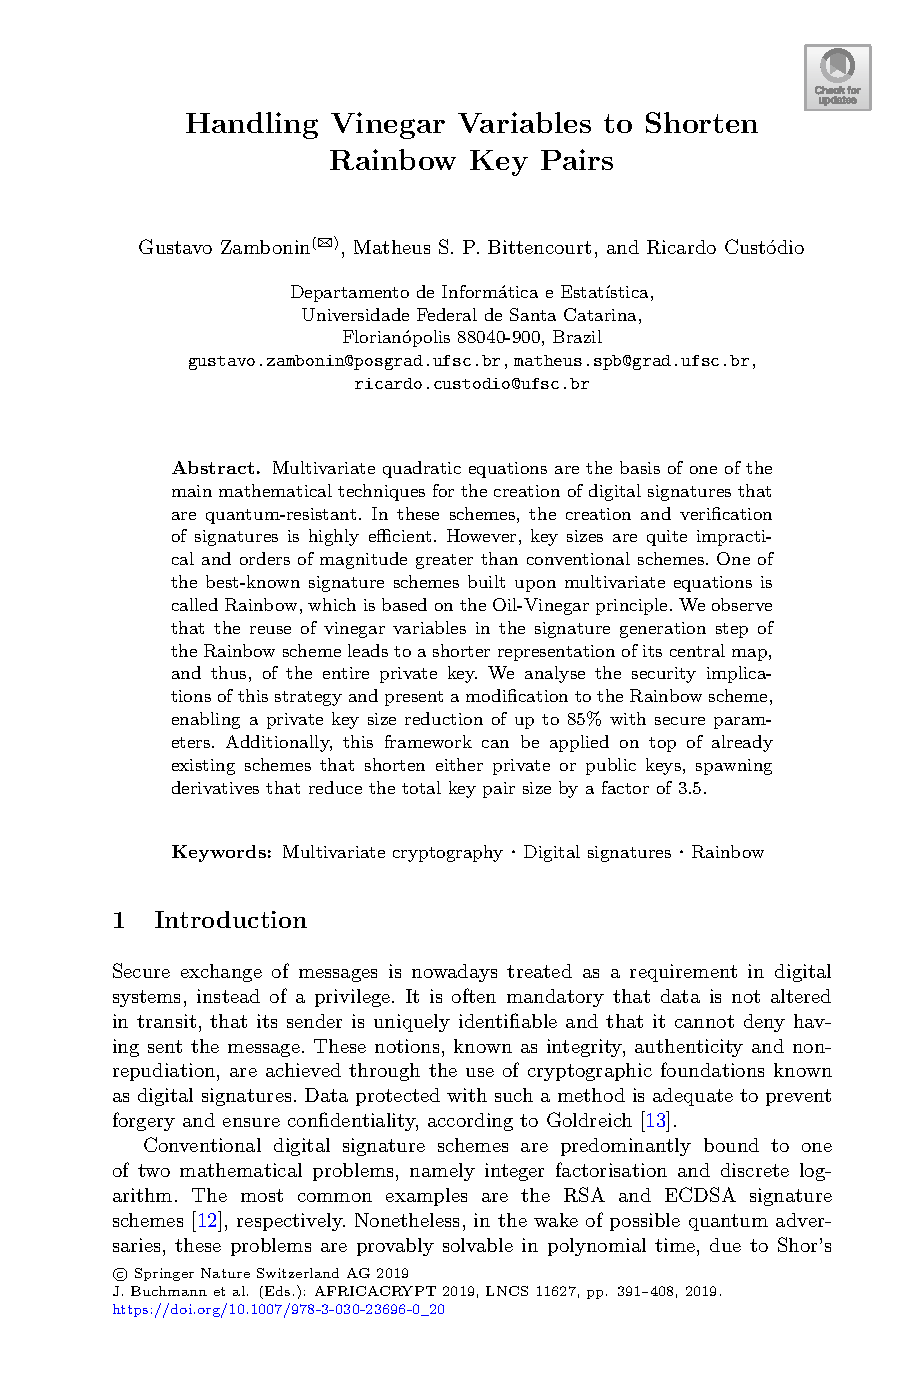
\includepdf[pages=-]{rainbow-eta.pdf}

\bibliographystyle{abnt-alf}
\bibliography{ref}

\end{document}
